\section{Modelo SM-CFHR}\label{sec:modelo}

El estimador \textbf{SM-CFHR} (\textit{Structured Monotone Capacity-Factor Huber Regressor}) opera íntegramente en el espacio adimensional del factor de capacidad y convierte sus predicciones a energía física únicamente al finalizar la inferencia. La Figura~\ref{fig:sm_cfhr_arq} resume el flujo matemático completo desde las magnitudes físicas hasta la reconstrucción energética.

\begin{figure}[!htbp]
\centering
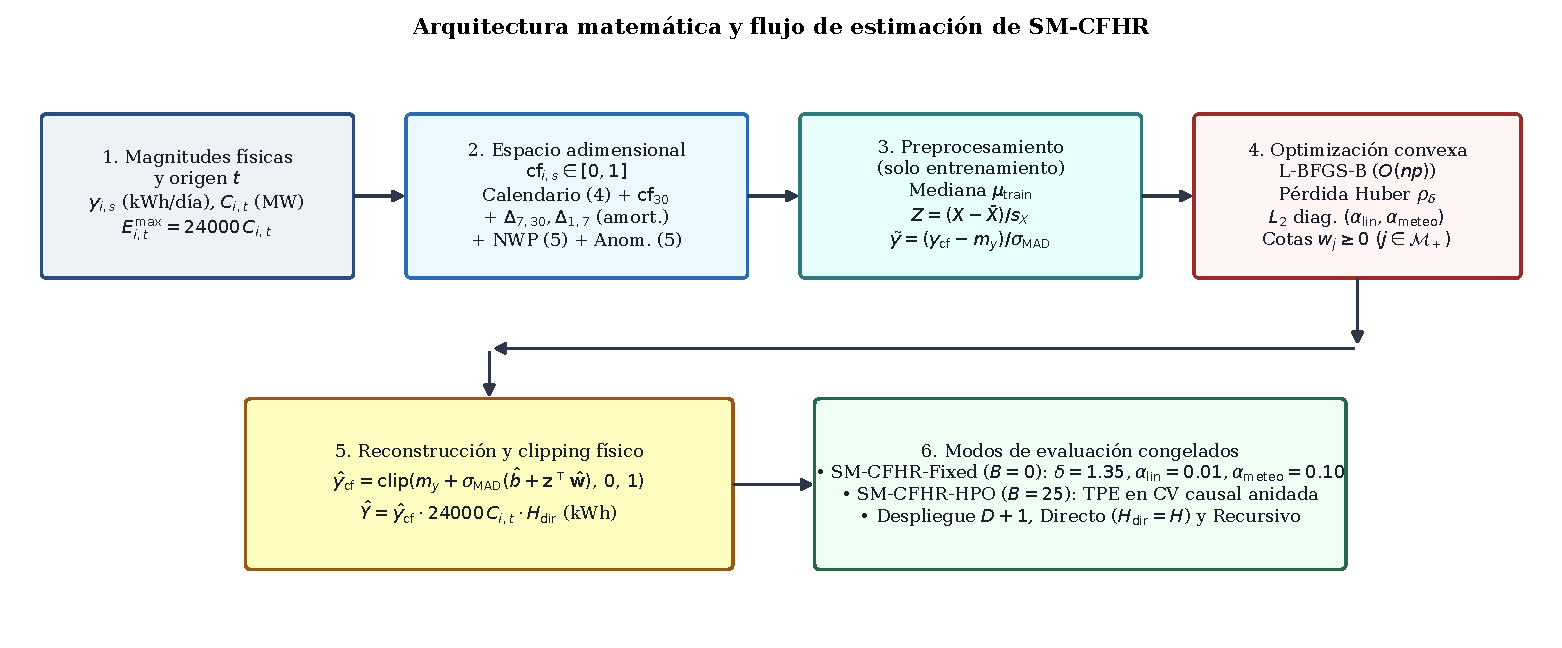
\includegraphics[width=0.98\textwidth]{figures/fig_sm_cfhr_arquitectura.pdf}
\caption{Flujo matemático de SM-CFHR: normalización causal por capacidad vigente, preprocesamiento en entrenamiento, optimización convexa L-BFGS-B con pérdida de Huber y $L_2$ diferenciada, y reconstrucción física.}
\label{fig:sm_cfhr_arq}
\end{figure}

\subsection{Representación causal de entrada}

Para una fila asociada a la planta $i$, origen de emisión $t$ y paso de adelanto $h \ge 1$ (fecha objetivo $t+h$), la función \texttt{extract\_cf\_features} construye un vector de predictores $\mathbf{x}_{i,t+h \mid t} \in \mathbb{R}^p$ a partir de las estadísticas causales disponibles en $\mathcal{F}_{i,t}$. Sea $E^{\max}_{i,t} = 24\,000\,C_{i,t}$ el denominador energético al origen, donde $C_{i,t}$ es la capacidad efectiva neta vigente (\texttt{cap\_MW\_D}). Denotando por $\bar{y}^{(30)}_{i,t}$, $\bar{y}^{(7)}_{i,t}$ y $y^{\mathrm{ult}}_{i,t}$ la media móvil de $30$ días (\texttt{media30\_kwh}), la media móvil de $7$ días (\texttt{media7\_kwh}) y la generación del último día válido (\texttt{kwh\_D}), los factores de capacidad históricos acotados se obtienen secuencialmente mediante:
\begin{equation}
\mathrm{cf}_{30} := \clip\!\left(\frac{\bar{y}^{(30)}_{i,t}}{E^{\max}_{i,t}}, 0, 1\right),\quad
\mathrm{cf}_{7} := \clip\!\left(\frac{\bar{y}^{(7)}_{i,t}}{E^{\max}_{i,t}}, 0, 1\right),\quad
\mathrm{cf}_{1} := \clip\!\left(\frac{y^{\mathrm{ult}}_{i,t}}{E^{\max}_{i,t}}, 0, 1\right),
\end{equation}
con respaldos causales jerárquicos ante valores no finitos: $\mathrm{cf}_{30} \leftarrow 0{,}15$, $\mathrm{cf}_{7} \leftarrow \mathrm{cf}_{30}$ y $\mathrm{cf}_{1} \leftarrow \mathrm{cf}_{7}$.

En los escenarios sin meteorología ($p = 7$), el vector de características $\mathbf{x}_{i,t+h \mid t}$ se compone de cuatro armónicos de calendario evaluados sobre la fecha objetivo $t+h$ ---$\sin(2\pi m/12)$, $\cos(2\pi m/12)$, $\sin(2\pi\,\mathrm{doy}/365{,}25)$ y $\cos(2\pi\,\mathrm{doy}/365{,}25)$--- seguidos de tres términos de dinámica autorregresiva en factor de capacidad:
\begin{equation}
x_5 = \mathrm{cf}_{30},\qquad
x_6 = \gamma_h (\mathrm{cf}_{7} - \mathrm{cf}_{30}),\qquad
x_7 = \gamma_h (\mathrm{cf}_{1} - \mathrm{cf}_{7}),
\label{eq:features_din}
\end{equation}
donde $\gamma_h := 0{,}85^{h-1}$ es el factor de amortiguamiento geométrico dependiente del paso de adelanto (\texttt{LEAD\_DAMPING = 0.85}). Durante el entrenamiento sobre observaciones pasadas, el ajuste se realiza con $h=1$ ($\gamma_1 = 1$), mientras que en el despliegue recursivo multihorizonte $\gamma_h$ atenúa progresivamente las desviaciones transitorias de corto plazo respecto al nivel base de $30$ días.

Cuando el escenario incorpora información meteorológica ($p = 17$), se concatenan diez predictores adicionales: cinco variables de pronóstico NWP ($\mathbf{z}_{i,t+h \mid t}$: irradiación horizontal \texttt{rad\_pron}, temperatura a $2\text{ m}$ \texttt{temp\_pron}, nubosidad \texttt{nube\_pron}, humedad relativa \texttt{humedad\_pron} y viento \texttt{viento\_pron}) y cinco anomalías causales ($\mathbf{a}_{i,t+h \mid t} = \mathbf{z}_{i,t+h \mid t} - \bar{\mathbf{z}}^{(30)}_{i,t}$), calculadas restando a cada variable pronosticada su media móvil de $30$ días estrictamente anterior a la emisión ($\le t$). El Apéndice~\ref{ap:escenarios} detalla el inventario completo de las $17$ variables.

\subsection{Preprocesamiento en entrenamiento y escalado robusto MAD}

Sea $\mathcal{D}_{\mathrm{train}} = \{(\mathbf{x}_k, y_k)\}_{k=1}^n$ el conjunto de entrenamiento válido del pliegue (filtrando filas con $E^{\max}_{k} > 0$ y objetivo finito), con matriz de predictores $X \in \mathbb{R}^{n \times p}$ y vector de factores de capacidad objetivo $\mathbf{y} \in [0,1]^n$ definido por \eqref{eq:cf_diario}. Toda transformación estadística se estima exclusivamente sobre $\mathcal{D}_{\mathrm{train}}$:
\begin{enumerate}
    \item \textbf{Imputación por mediana:} si algún predictor presenta valores no finitos, se reemplaza por la mediana por columna $\mu_j = \mathrm{mediana}_k(X_{kj})$ calculada en $\mathcal{D}_{\mathrm{train}}$ (con respaldo $0{,}0$ si toda la columna es faltante), obteniendo $X^{\mathrm{imp}}$.
    \item \textbf{Estandarización de predictores:} se calculan la media muestral $\bar{x}_j = \frac{1}{n}\sum_{k=1}^n X^{\mathrm{imp}}_{kj}$ y la desviación estándar poblacional $s_j = \big(\frac{1}{n}\sum_{k=1}^n (X^{\mathrm{imp}}_{kj} - \bar{x}_j)^2\big)^{1/2}$. Para evitar divisiones inestables en columnas constantes o cuasi-degeneradas, la escala efectiva es $\tilde{s}_j = s_j$ si $s_j > 10^{-8}$ y $\tilde{s}_j = 1$ en caso contrario, produciendo la matriz estandarizada $Z \in \mathbb{R}^{n \times p}$ con entradas $Z_{kj} = (X^{\mathrm{imp}}_{kj} - \bar{x}_j)/\tilde{s}_j$.
    \item \textbf{Escalado robusto de la respuesta:} para que el umbral $\delta$ de la pérdida de Huber actúe en unidades adimensionales comparables entre plantas y estaciones, la respuesta se centra y escala mediante la mediana $m_y = \mathrm{mediana}(\mathbf{y})$ y la desviación absoluta mediana $\mathrm{MAD}(\mathbf{y}) = \mathrm{mediana}(|\mathbf{y} - m_y|)$:
    \begin{equation}
    \sigma_y := \begin{cases}
    \max\{1{,}4826\,\mathrm{MAD}(\mathbf{y}),\; 10^{-6}\} & \text{si } \mathrm{MAD}(\mathbf{y}) > 0, \\
    \max\{\operatorname{std}(\mathbf{y}),\; 10^{-6}\} & \text{si } \mathrm{MAD}(\mathbf{y}) = 0,
    \end{cases}
    \qquad
    \tilde{y}_k := \frac{y_k - m_y}{\sigma_y}.
    \label{eq:mad_scale}
    \end{equation}
    La constante $1{,}4826 = 1/\Phi^{-1}(0{,}75)$ hace consistente a $\sigma_y$ con la desviación estándar bajo normalidad, preservando un punto de ruptura del $50\%$ \cite{rousseeuw1993mad}.
\end{enumerate}

\subsection{Función objetivo, regularización estructurada y restricciones de signo}

Sobre los predictores estandarizados $\mathbf{z}_k \in \mathbb{R}^p$ y la respuesta escalada $\tilde{y}_k \in \mathbb{R}$, SM-CFHR busca un intercepto no penalizado $b \in \mathbb{R}$ y un vector de coeficientes $\mathbf{w} \in \mathbb{R}^p$ que minimicen la suma de la pérdida promedio de Huber y una penalización cuadrática diagonal diferenciada:
\begin{equation}
\min_{b \in \mathbb{R},\; \mathbf{w} \in \mathcal{C}} \; J(b, \mathbf{w}) := \frac{1}{n}\sum_{k=1}^{n} \rho_\delta\!\left(\tilde{y}_k - b - \mathbf{z}_k^\top \mathbf{w}\right) + \frac{1}{2}\mathbf{w}^\top D_\alpha \mathbf{w},
\label{eq:objetivo_smcfhr}
\end{equation}
donde $\rho_\delta : \mathbb{R} \to \mathbb{R}_{\ge 0}$ es la pérdida de Huber con umbral $\delta > 0$,
\begin{equation}
\rho_\delta(r) := \begin{cases}
\frac{1}{2} r^2 & \text{si } |r| \le \delta, \\
\delta\left(|r| - \frac{1}{2}\delta\right) & \text{si } |r| > \delta,
\end{cases}
\label{eq:huber}
\end{equation}
la matriz diagonal de regularización $D_\alpha = \diag(d_1,\dots,d_p)$ asigna penalizaciones por familia de predictores,
\begin{equation}
d_j := \begin{cases}
\alpha_{\mathrm{meteo}} & \text{si } j \in \mathcal{G}_{\mathrm{meteo}} \text{ y } \texttt{structured}=\texttt{True}, \\
\alpha_{\mathrm{lin}} & \text{en caso contrario},
\end{cases}
\label{eq:d_alpha}
\end{equation}
siendo $\mathcal{G}_{\mathrm{meteo}} = \{8,\dots,17\}$ el bloque de diez variables meteorológicas y anomalías (vacío cuando no hay meteorología), y el conjunto factible $\mathcal{C} \subseteq \mathbb{R}^p$ impone restricciones de signo no negativo sobre el subconjunto de índices físicamente monótonos $\mathcal{M}_+$:
\begin{equation}
\mathcal{C} := \{\mathbf{w} \in \mathbb{R}^p : w_j \ge 0 \;\forall j \in \mathcal{M}_+\},
\quad
\mathcal{M}_+ = \begin{cases}
\{\mathrm{cf}_{30}, \mathrm{rad\_pron}\} & \text{con clima}, \\
\{\mathrm{cf}_{30}\} & \text{sin clima}.
\end{cases}
\label{eq:conjunto_factible}
\end{equation}

Desde el punto de vista estadístico, \eqref{eq:objetivo_smcfhr} extiende la regresión Ridge clásica \cite{hoerl1970} y los híbridos robustos analizados por Owen~\cite{owen2007} en dos direcciones específicas del problema fotovoltaico. Por un lado, la matriz anisotrópica $D_\alpha$ permite aplicar una contracción moderada ($\alpha_{\mathrm{lin}}$) a la dinámica autorregresiva y estacional mientras contrae con mayor severidad ($\alpha_{\mathrm{meteo}}$) las variables NWP, evitando que errores meteorológicos de mediano plazo sobreajusten el modelo; ello no implica que $\alpha_{\mathrm{meteo}} > \alpha_{\mathrm{lin}}$ reduzca el error en todos los regímenes, sino que introduce un grado de libertad interpretable controlado por validación. Por otro lado, las cotas $w_j \ge 0$ para $j \in \mathcal{M}_+$ garantizan que, a igualdad de los demás predictores, un mayor nivel reciente de factor de capacidad o una mayor irradiación pronosticada no produzcan pendientes negativas espurias por colinealidad.

Es importante distinguir entre los elementos estructurales fijos y los hiperparámetros de ajuste. Aunque la clase subyacente \texttt{AdaptiveStructuredHuberRegressor} admite expansiones por splines y términos bilineales en un selector interno heredado, el protocolo congelado de SM-CFHR fija explícitamente \texttt{n\_knots=0}, \texttt{max\_interactions=0}, \texttt{anchor="none"}, \texttt{structured=True} y \texttt{use\_mono=True}. Con ello se definen dos variantes experimentales comparables:
\begin{itemize}
    \item \textbf{SM-CFHR-Fixed ($B=0$):} configuración congelada con $\delta = 1{,}35$, $\alpha_{\mathrm{lin}} = 0{,}01$ y $\alpha_{\mathrm{meteo}} = 0{,}10$ (en ausencia de meteorología, $d_j = \alpha_{\mathrm{lin}}$ para todo $j$), sin búsqueda interna de hiperparámetros.
    \item \textbf{SM-CFHR-HPO ($B=25$):} optimización bayesiana TPE mediante Optuna dentro de cada pliegue externo sobre el espacio continuo $\delta \in [0{,}5, 3{,}0]$, $\alpha_{\mathrm{lin}} \in [10^{-4}, 1{,}0]$ (escala logarítmica) y, cuando hay meteorología, $\alpha_{\mathrm{meteo}} \in [10^{-3}, 10{,}0]$ (escala logarítmica).
\end{itemize}

\subsection{Reconstrucción física y despliegue multihorizonte}

Dado un vector de consulta $\mathbf{x}_q$ con versión imputada y estandarizada $\mathbf{z}_q = (\mathbf{x}^{\mathrm{imp}}_q - \bar{\mathbf{x}})/\tilde{\mathbf{s}}$ usando los parámetros de entrenamiento, el modelo ajustado $(\hat{b}, \hat{\mathbf{w}})$ produce la predicción en factor de capacidad acotada físicamente:
\begin{equation}
\widehat{\mathrm{cf}}_q := \clip\!\left(m_y + \sigma_y \big(\hat{b} + \mathbf{z}_q^\top \hat{\mathbf{w}}\big),\; 0,\; 1\right),
\qquad
\hat{y}_q := \widehat{\mathrm{cf}}_q \cdot 24\,000\,C_{i,t} \cdot H_{\mathrm{dir}} \quad (\text{kWh}),
\label{eq:pred_fisica}
\end{equation}
con respaldo al promedio histórico $\bar{y}^{(30)}_{i,t}\,H_{\mathrm{dir}}$ si la capacidad al origen no fuera finita, seguido de un último acotamiento al intervalo $[0, 24\,000\,H_{\mathrm{dir}}\,C_{i,t}]$.

La Figura~\ref{fig:despliegue_mh} contrasta los tres modos de despliegue implementados en \texttt{oof\_runner.py}:
\begin{enumerate}
    \item \textbf{Pronóstico $D+1$ ($H=1$, $H_{\mathrm{dir}}=1$):} evalúa \eqref{eq:pred_fisica} una sola vez para $t+1$.
    \item \textbf{Esquema directo acumulado ($H \in \{7,14,21,28\}$, $H_{\mathrm{dir}}=H$):} entrena sobre ventanas completas cuya fecha final cumple $t_{\mathrm{end}} = t_{\mathrm{origen}} + H \le t_0$ y predice $\hat{Y}_{i,t_0}^{(H)}$ en un único paso sin realimentación.
    \item \textbf{Esquema recursivo multihorizonte ($H \in \{7,14,21,28\}$, $H_{\mathrm{dir}}=1$):} inicializa al origen $t_0$ el objeto causal \texttt{PlantRecursiveState} (o \texttt{PlantRecursiveWeatherState} con GEFSv12), fijando $C_{i,t_0}$ y la línea base climática de $30$ días. Para cada $h = 1,\dots,H$, construye las características de consulta para $t_0 + h$ usando $\gamma_h = 0{,}85^{h-1}$ y el pronóstico GEFSv12 emitido en $t_0$ para $t_0 + h$, obtiene $\hat{y}_{i,t_0+h \mid t_0}$ mediante \eqref{eq:pred_fisica}, e inserta exclusivamente dicha predicción propia en el búfer circular de la planta para actualizar las medias móviles $\bar{y}^{(7)}$ y $\bar{y}^{(30)}$ antes del paso $h+1$.
\end{enumerate}

En la versión congelada \texttt{v1.0.2} existía un matiz entre el despliegue externo (actualización exacta de ventanas deslizantes sobre el búfer histórico) y la validación interna de HPO (actualización exponencial aproximada). A partir de la versión \texttt{v1.0.3} (\texttt{HPO\_PROTOCOL\_VERSION = v1.0.3-exact-recursive-state}), la validación interna de Optuna TPE delega directamente en la misma función \texttt{rollout\_recursive\_from\_origin} basada en \texttt{PlantRecursiveState} y \texttt{PlantRecursiveWeatherState}, garantizando equivalencia causal exacta con el despliegue externo y rechazando automáticamente estudios SQLite heredados de \texttt{v1.0.2}. Asimismo, es crucial subrayar que, aunque el ajuste interno \eqref{eq:objetivo_smcfhr} es un problema convexo, la composición recursiva de $H$ pasos realimentando $\hat{y}_{i,t_0+h \mid t_0}$ es una función no lineal y no convexa de los parámetros.

\begin{figure}[!htbp]
\centering
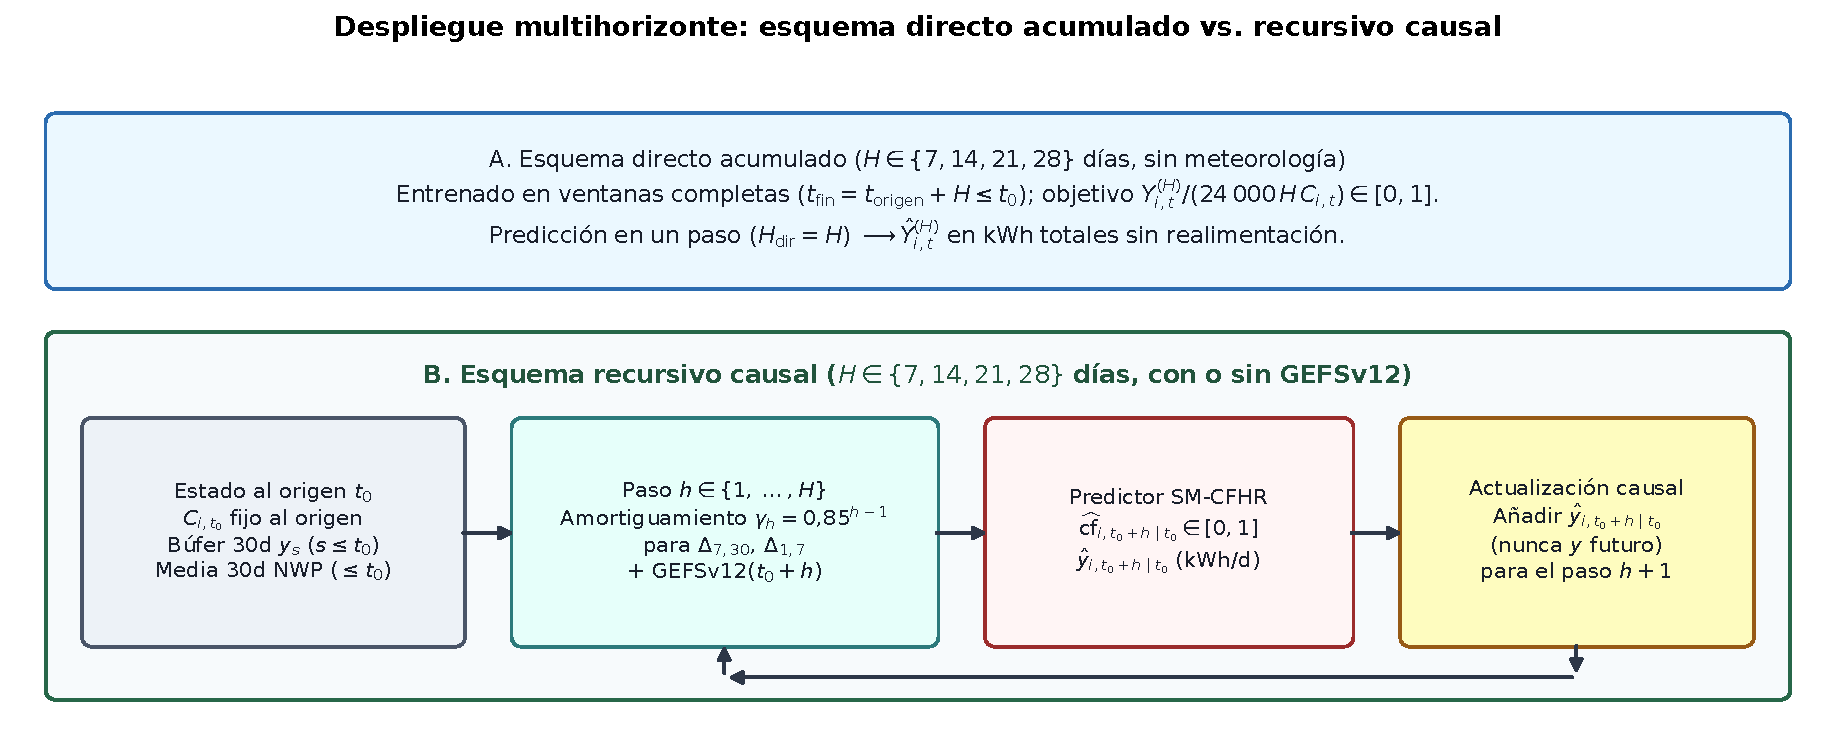
\includegraphics[width=0.98\textwidth]{figures/fig_despliegue_multihorizonte.pdf}
\caption{Comparación estructural entre el esquema directo acumulado ($H_{\mathrm{dir}}=H$, sin realimentación) y el despliegue recursivo multihorizonte con actualización causal mediante predicciones propias y amortiguamiento geométrico.}
\label{fig:despliegue_mh}
\end{figure}
